\chapter{Pattern Learning}

\section{Introduction}

Here in pattern learning, we extract the common pattern from a set of ARGs, and the extracted information can then be used to summarize the given ARGs and predict if a new ARG contains the common pattern we summarized. In our work, for instance, we can extract the common structure of a set of proteins that share the same function. The common structure we extracted can give us insight on how this structure can perform such function, and if a new protein also has the same structure that can carry out the same function.\\

To perform pattern learning, we utilize a probabilistic parametric model to represent the common pattern from the graphs (Hong\footnotemark and Huang 2004). Similar to how three normal distribution (or components) can capture the data distribution generated by $f(x)$ below, we used a couple component ARGs with various mean and variance to represent the common pattern:
\footnotetext{My dear advisor!}

\begin{figure}[h]
	\centering
	\captionsetup{justification=centering}
	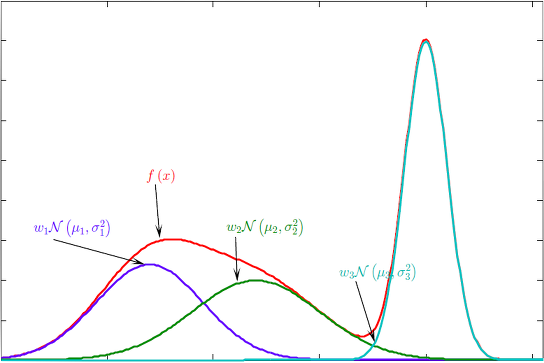
\includegraphics[width=0.65\textwidth]{figs/mixture.png}
	\caption[Caption for LOF]{\emph{The data distribution generated by $f(x)$ can be captured by three normal distribution with various means and variances.}}
	\label{fig:mixture}
\end{figure}

Therefore, the model training process is essentially training and setting up some component ARGs so that all the nodes and edges have the means and variances that best capture the common pattern in the given set of ARGs.\\

Based on the algorithm described by Hong and Huang, we first pick some ARGs from the input sample ARGs, and initialize them as the component ARGs. Then we perform an EM algorithm where on the \textbf{E}xpectation step we run the graph matching algorithm to calculate the matching probability between model ARGs and sample ARGs while on the \textbf{M}aximization step we update the model ARG (e.g. updating means, variances, and deleting redundant nodes) in order to achieve higher matching probability. Finally, once the update is very small, we output the model ARGs to represent the common pattern in sample ARGs:\\

\begin{figure}[h]
	\centering
	\captionsetup{justification=centering}
	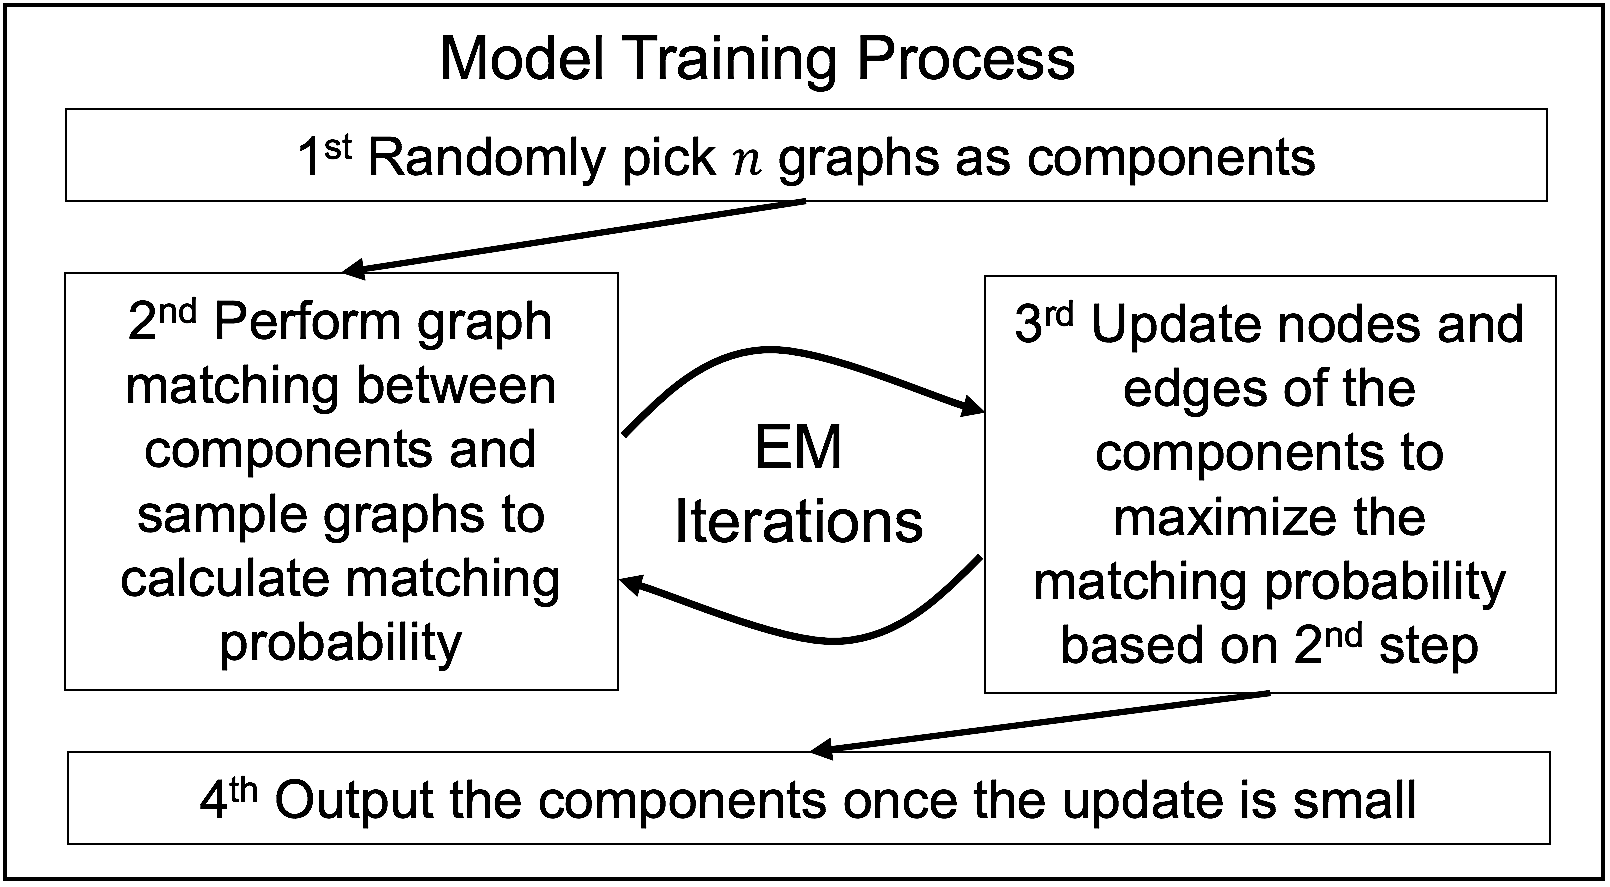
\includegraphics[width=0.8\textwidth]{figs/model_training.png}
	\caption[Caption for LOF]{\emph{The probabilistic parametric model training process with EM algorithm.}}
	\label{fig:model_training}
\end{figure}

\section{Syntax and Definition}

The sample ARGs (i.e. the set of ARGs we want to learn/extract pattern from) is denoted as $\{G_s\}_{s=1}^S$ where $S$ is the number of model components. Within each sample ARG, we indicate the label for each node and edge as $\overrightarrow{N^s_a}$ and $\overrightarrow{E^s_{ab}}$. This is similar to what we have in Chapter \ref{chap: graphmatching} but with an additional index $s$ indicating which sample $G$ these nodes and edges belong to. In addition, we denoted the real nodes in sample ARG, $G_s-\phi$, as $\widehat{G_s}$.\\

For the model, we denoted it as $Z$ and the model consists of a set of parametric model components $\{\Phi_w\}_{w=1}^W$ where $W$ is the number of model components. For each component, there are also an associated weight $\alpha_w$ which indicates how much information the component captures and how important the component is.\\

Within each component ARG, we indicate the mean for each node and edge as $\overrightarrow{N^w_a}$ and $\overrightarrow{E^w_{ab}}$ similar to what we have for sample ARGs, but with $w$ instead of $s$ indicating which model this node and edge belongs to. In addition to the mean, there are also the covariance matrixes for node and edge denoted by $\Sigma^w_a$ and $\Sigma^w_{ab}$ with a similar index. Last but not least, for each node in each component, there is an associated frequency/weight $\beta^w_a$ indicating how important one node is and if we can delete such node.\\

In addition, the matching algorithm introduced in Chapter \ref{chap: graphmatching} can generate match matrix $M^{sw}$ between sample ARG $G_s$ and component ARG $\Phi_w$ as well as the associated node/edge compatibility $C^{sw}$.

\section{Problem Definition}

Given a set of sample ARG $\{G_s\}_{s=1}^S$, our problem will be inferring the parameters in $Z$ including the number of components $W$, weight for each component $\alpha$, mean for each node/edge $\overrightarrow{N^w}$/$\overrightarrow{E^w}$, and the covariance associated with them $\Sigma$.\\

\begin{figure}[h]
	\centering
	\captionsetup{justification=centering}
	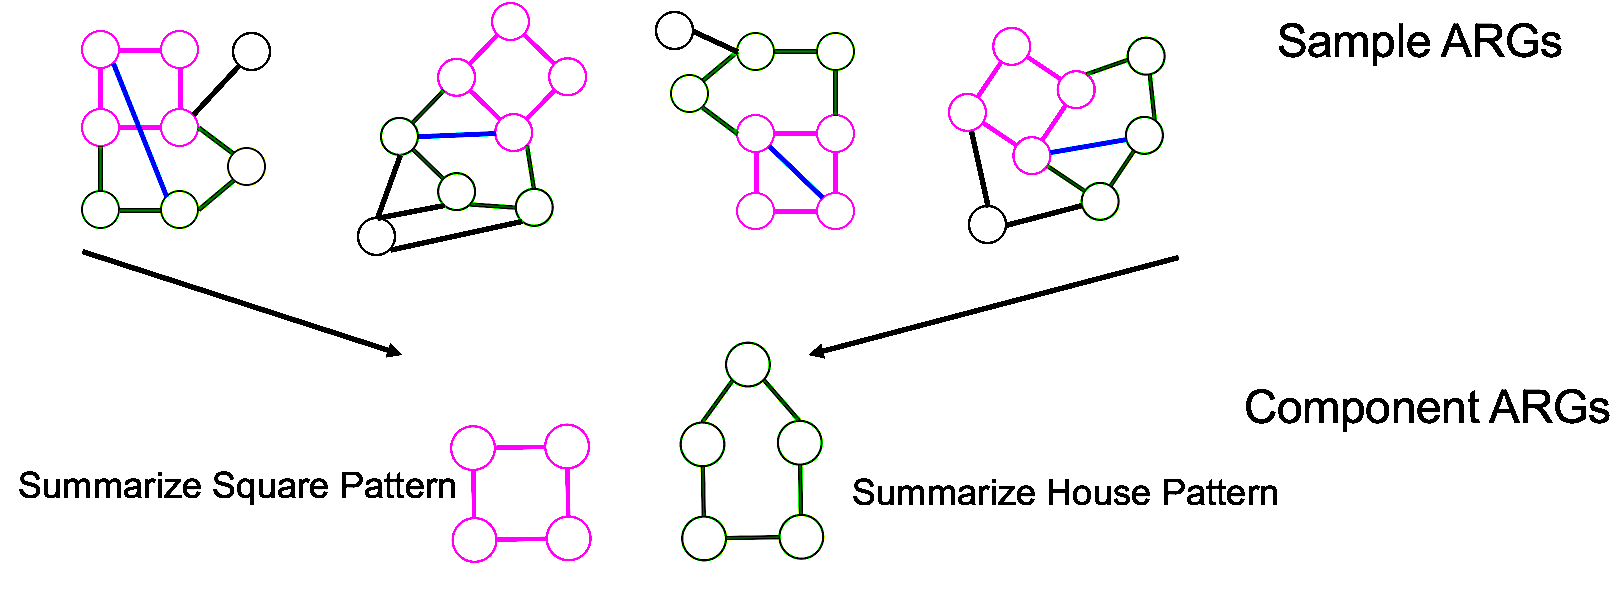
\includegraphics[width=0.8\textwidth]{figs/component_summary.png}
	\caption[Caption for LOF]{\emph{Component can summarize different part of the common pattern.}}
	\label{fig:component_summary}
\end{figure}

\section{Initializing the Components}

The first step of training the model is initializing the components in the model.\\

The way we do is manually pick $W$ random ARG from our sample set, and initialize them as component ARG $\Phi$. We took their original label as the mean, set their covariance matrix as the identity matrix $I$, and give equal weight to all the components and nodes. If we are converting a sample $G_s$ to a component $\Phi_w$, we would have:

\begin{align} 
\overrightarrow{N^w_a} & \leftarrow \overrightarrow{N^s_a} & \forall a \in \widehat{G_s}\\
\overrightarrow{E^w_{ab}} & \leftarrow \overrightarrow{E^s_{ab}}& \forall a,b \in \widehat{G_s}\\
\Sigma^w_a & \leftarrow  I\\
\Sigma^w_b  & \leftarrow  I\\
\alpha_w & \leftarrow \frac{1}{W}\\
\beta^w_a & \leftarrow \frac{1}{|G_s|}& \forall a \in G_s)
\end{align}\\

While we pick $W$ manually based on the complexity of the pattern here, theoretically, we can also start with a relatively larger number of components are delete some of them later. In terms of picking the sample, you can also do better than random by doing a pairwise graph matching among the sample ARG and choose ones that are the most representative based on the match matrixes $M$.

\newpage

\section{EM Algorithm}

Once we initialized the components $\{\Phi_w\}_{w=1}^W$ with all the parameters, we will then run through an EM algorithm to tune this parameters so our model $Z$ can capture the sample $\{G_s\}_{s=1}^S$ at its best. EM algorithm consist of an estimation step where we estimate how well our parameters perform and a maximization step where we tune the parameters to maximize the estimation. We run through these two steps iteratively until the tuning on the parameter is very small.

\subsection{Estimation Step}

In this step we estimate how well model $Z$ representing the sample ARG $G$ as $P(G|Z)$. Once we finish training the model, $f(G_{new}|Z)$ can also be used to predict if a new ARG $G_{new}$ contains the learned/extracted pattern. \\

The first thing we do in the estimation step is matching each component $\Phi_w$ with each sample $G_s$, and get a match matrix $M^{sw}$ from the graph matching algorithm introduced in Chapter \ref{chap: graphmatching}. In addition, the algorithm will also return the node and edge compatibility $C^{sw}$ computed as described in Section \ref{ssec:compatibility}.\\

Once we have the match matrix, we can calculate the probability of $G_s$ matching $\Phi_w$:

\begin{align} 
& \xi(G_s|\Phi_w)=\sum_{a=1}^{\widehat{G_s}}\sum_{i=1}^{\Phi_w}M^{sw}_{ai}C^{sw}_{ai}+ \sum_{a=1}^{\widehat{G_s}}\sum_{b=1}^{\widehat{G_s}}\sum_{i=1}^{\Phi_w}\sum_{j=1}^{\Phi_w}M^{sw}_{ai}M^{sw}_{bj}C^{sw}_{abij}\\
& P(G_s=\Phi_w)=\frac{\xi(G_s|\Phi_w)}{\sum_{t=1}^{W}\xi(G_s|\Phi_t)}
\end{align}\\

With $\xi(G_s|\Phi_w)$, we then can calculate:

\begin{equation} 
f(G|Z) = \sum_{w=1}^W\alpha_w\xi(G|\Phi_w) \label{eq:fgz}
\end{equation}\\

\subsection{Maximization Step}

In the maximization step, we adjust and tune the variable based on $P(G_s=\Phi_w)$, $M^{sw}$ and $C^{sw}$ that we calculated in the Estimation step.

\subsubsection{Update Component Weight}

First we update the component weight $\alpha_w$ for each component $\Phi_w$ as:

\begin{equation} 
\alpha_w=\frac{\sum^S_{s=1}P(G_s=\Phi_w)}{S}
\end{equation}\\

The component weight here is essentially calculating the average probability it matched to all the sample ARGs $\{G_s\}^S_{s=1}$.

\subsubsection{Update Component Node Frequency}

Then we update the frequency (i.e. weight) for each node in each component $\Phi_w$:

\begin{equation} 
\beta^w_a=\frac{\sum^S_{s=1}\sum^{\widehat{G_s}}_{i=1}M^{sw}_{ia}P(G_s=\Phi_w)}{\sum^S_{s=1}|\widehat{G_s}|P(G_s=\Phi_w)}
\end{equation}\\

The component node frequency is essentially an weighted average of the matching probability of this specific component node in all the matching matrix $M^{sw}$.\\

\subsubsection{Update Mean for Component Node}

To tune the mean for each component node, $\overrightarrow{N^w_a}$, we follow:

\begin{equation} 
\overrightarrow{N^w_a}=\frac{\sum^S_{s=1}\sum^{\widehat{G_s}}_{i=1}\overrightarrow{N^s_i}M^{sw}_{ia}P(G_s=\Phi_w)}{\sum^S_{s=1}\sum^{\widehat{G_s}}_{i=1}M^{sw}_{ia}P(G_s=\Phi_w)}
\end{equation}\\

Here we essentially calculated a weighted average of all the sample nodes, $\overrightarrow{N^s_i}$, based on how likely our component node matches to that sample node in match matrix $M^{sw}$ and how likely the component matches to that sample $P(G_s=\Phi_w)$.\\

\subsubsection{Update Covariance Matrix for Component Node}

Once we update the mean, we will also need to update the covariance matches $\Sigma^w_a$ for the component node:

\begin{equation} 
\Sigma^w_a=\frac{\sum^S_{s=1}\sum^{\widehat{G_s}}_{i=1}\overrightarrow{x^s_i}\overrightarrow{x^s_i}^TM^{sw}_{ia}P(G_s=\Phi_w)}{\sum^S_{s=1}\sum^{\widehat{G_s}}_{i=1}M^{sw}_{ia}P(G_s=\Phi_w)}
\end{equation}
where $\overrightarrow{x^s_i} = \overrightarrow{N^s_i} - \overrightarrow{N^w_a}$.\\

Similarly, here we essentially calculated a weighted average of covariance between the component node and sample nodes, $(\overrightarrow{N^s_i} - \overrightarrow{N^w_a})(\overrightarrow{N^s_i} - \overrightarrow{N^w_a})^T$, based on how likely our component node matches to that sample node in match matrix $M^{sw}$ and how likely the component matches to that sample $P(G_s=\Phi_w)$.\\

\subsubsection{Update Mean for Component Edge}

Similar to how we calculate the mean for component node $overrightarrow{N^w_a}$, we calculate the mean for component edge $\overrightarrow{E^w_{ab}}$ as:

\begin{equation} 
\overrightarrow{E^w_{ab}}=\frac{\sum^S_{s=1}\sum^{\widehat{G_s}}_{i=1}\sum^{\widehat{G_s}}_{j=1}\overrightarrow{E^s_{ij}}M^{sw}_{ia}M^{sw}_{bj}P(G_s=\Phi_w)}{\sum^S_{s=1}\sum^{\widehat{G_s}}_{i=1}\sum^{\widehat{G_s}}_{j=1}M^{sw}_{ia}M^{sw}_{bj}P(G_s=\Phi_w)}
\end{equation}

\subsubsection{Update Covariance Matrix for Component Edge}

Similar to how we calculate the covariance matrix for component node $\Sigma^w_a$, we calculate the covariance matrix for component edge $\Sigma^w_{ab}$ as:

\begin{equation} 
\Sigma^w_{ab}=\frac{\sum^S_{s=1}\sum^{\widehat{G_s}}_{i=1}\sum^{\widehat{G_s}}_{j=1}\overrightarrow{z^s_{ij}}\overrightarrow{z^s_{ij}}^TM^{sw}_{ia}M^{sw}_{bj}P(G_s=\Phi_w)}{\sum^S_{s=1}\sum^{\widehat{G_s}}_{i=1}\sum^{\widehat{G_s}}_{j=1}M^{sw}_{ia}M^{sw}_{bj}P(G_s=\Phi_w)}
\end{equation}
where $\overrightarrow{z^s_{ij}} = \overrightarrow{E^s_{ij}} - \overrightarrow{E^w_{ab}}$.\\

\subsubsection{Delete Redundant Node}

Since we initialized the component from sample ARGs, it is likely that the component itself will have background nodes (i.e. nodes not in the common pattern) that are redundant. To reduce the component ARGs from sample ARGs to the smaller common pattern, we can do node deletion based on the node frequency $\beta^w_a$ and some threshold. For instance, we choose to delete the $a$th node in $\Phi_w$ if:

\begin{equation} 
\beta^w_a < 1 - 0.85^n
\end{equation}
where $n$ indicate the $n$th round of the EM algorithm.\\

However, you can also choose to used a hard threshold like $0.85$ or delete redundant node in the very last round. In addition, we can also choose to delete redundant component here, even though we did not explore such option.

\subsubsection{Converge Condition and EM Algorithm Exit}

At the beginning of the EM algorithm, the maximization step will make large modification on each parameter, so we would go back to the estimation step after finishing the maximization step. \\

However, towards the end of the algorithm, we need to check if the EM algorithm has already converged (changes are small). If so, then we can exit the EM algorithm and go to the next step. Here, we simply compared previous component weight $\alpha^{(0)}$ with the current component weight $\alpha^{(1)}$, and exit if the differences is smaller than some number $\iota$:

\begin{equation} 
\sum^{W}_{w=1}\alpha^{(0)}_w<\iota
\end{equation}\\

However, these are not the only choices, and you can use other converging conditions if you like.\\

\newpage

\section{Detect the Spatial Pattern}

Once we finished training the model, how do we detect or predict if the extracted/summarized pattern exist in a new ARG? As mentioned above, we can use $f(G|Z)$ calculated by Eq.\ref{eq:fgz} as our similarity score to determine if the new ARG, $G$, contains the same spatial pattern as the training samples. Therefore, we would need to setup some sort of threshold, $\chi$, so that $G$ contains the learned pattern only if $f(G|Z)>\chi$.\\ 

To setup $\chi$, we generate a set of $R$ random graphs $\{G^r\}^{R}_{r=1}$ with similar number of nodes, edge connectivity\footnotemark, and labels as our training sample $\{G^s\}^{S}_{s=1}$. With the random generated ARGs, we can calculate a set of similarity score $\{f(G^r|Z)\}^{R}_{r=1}$ that can help us determine the threshold $\chi$. If you have enough computational power, and are able calculate the similarity score for a very large number\footnotemark of random ARG. You can simply take the $99.99\%$ percentile of the similarity score set $\{f(G^r|Z)\}^{R}_{r=1}$.\\
\footnotetext{How many nodes one node connected to.} 

However, unlike Google\footnotemark, we do not live in a magic land. Therefore, we only calculated the similarity score for $50$ random ARGs and run z-test on the set of similarity scores $S=\{f(G^r|Z)\}^{R}_{r=1}$ which allows us to set the threshold $\chi$ as: 
$$\chi \leftarrow \mu+3\sigma$$
where $\mu$ and $\sigma$ are the mean and variance of the similarity scores of random ARGs.
\footnotetext{Let's say $R>1,000,000$.}
\footnotetext{https://twitter.com/deliprao/status/842635509255962624}

\section{Implementation Detail}

\subsection{Coding Complexity}

While the model introduced here seems to be pretty straight forward, the actual coding is rather tedious since we have many steps, parameters and nested summation. Therefore, we break down the algorithm and modulated each step so it is easier to debug.

\subsection{Null Node in the Model}

While it is not mentioned above, the model we implemented actually has a null node $\phi$, but it does not have any label on the node or edges. Instead, the graph matching algorithm will ignore this null node and used its own null node definition as described in Section \ref{ssec:nullnode}. However, when the graph matching return the match matrix and compatibility, $M^{sw}$ and $C^{sw}$, they include the value for algorithm's own null node which we can used for the model null node. Such implementation allows us to use the graph matching algorithm developed earlier with very little modification and save the troubles of maintaining the parameters for the null node.

\subsection{Run Time}

We trained a model with $2$ components on $5$ pattern embedded ARG with $\sim40$ nodes, and it took $\sim TBD$ minutes.\\

As mentioned in Section \ref{ssec:graphmatchingruntime}, you can adjust the parameter for converging condition and learning rate to tradeoff between accuracy and running time.

\section{Testing the Model}

Similar to how we generated test cases in Section \ref{sec:graphmatchingtest} for graph matching algorithm, we generate a set of ARGs with ($G^p$) or without ($G^r$ i.e. random ARG) the embedding pattern. \\

Then we train a model on some of the ARGs with the pattern (i.e. $G^p$) and plot a histogram of the similarity score ($f(G|Z)$) for all $G^p$ and $G^r$:

\begin{figure}[h]
	\centering
	\captionsetup{justification=centering}
	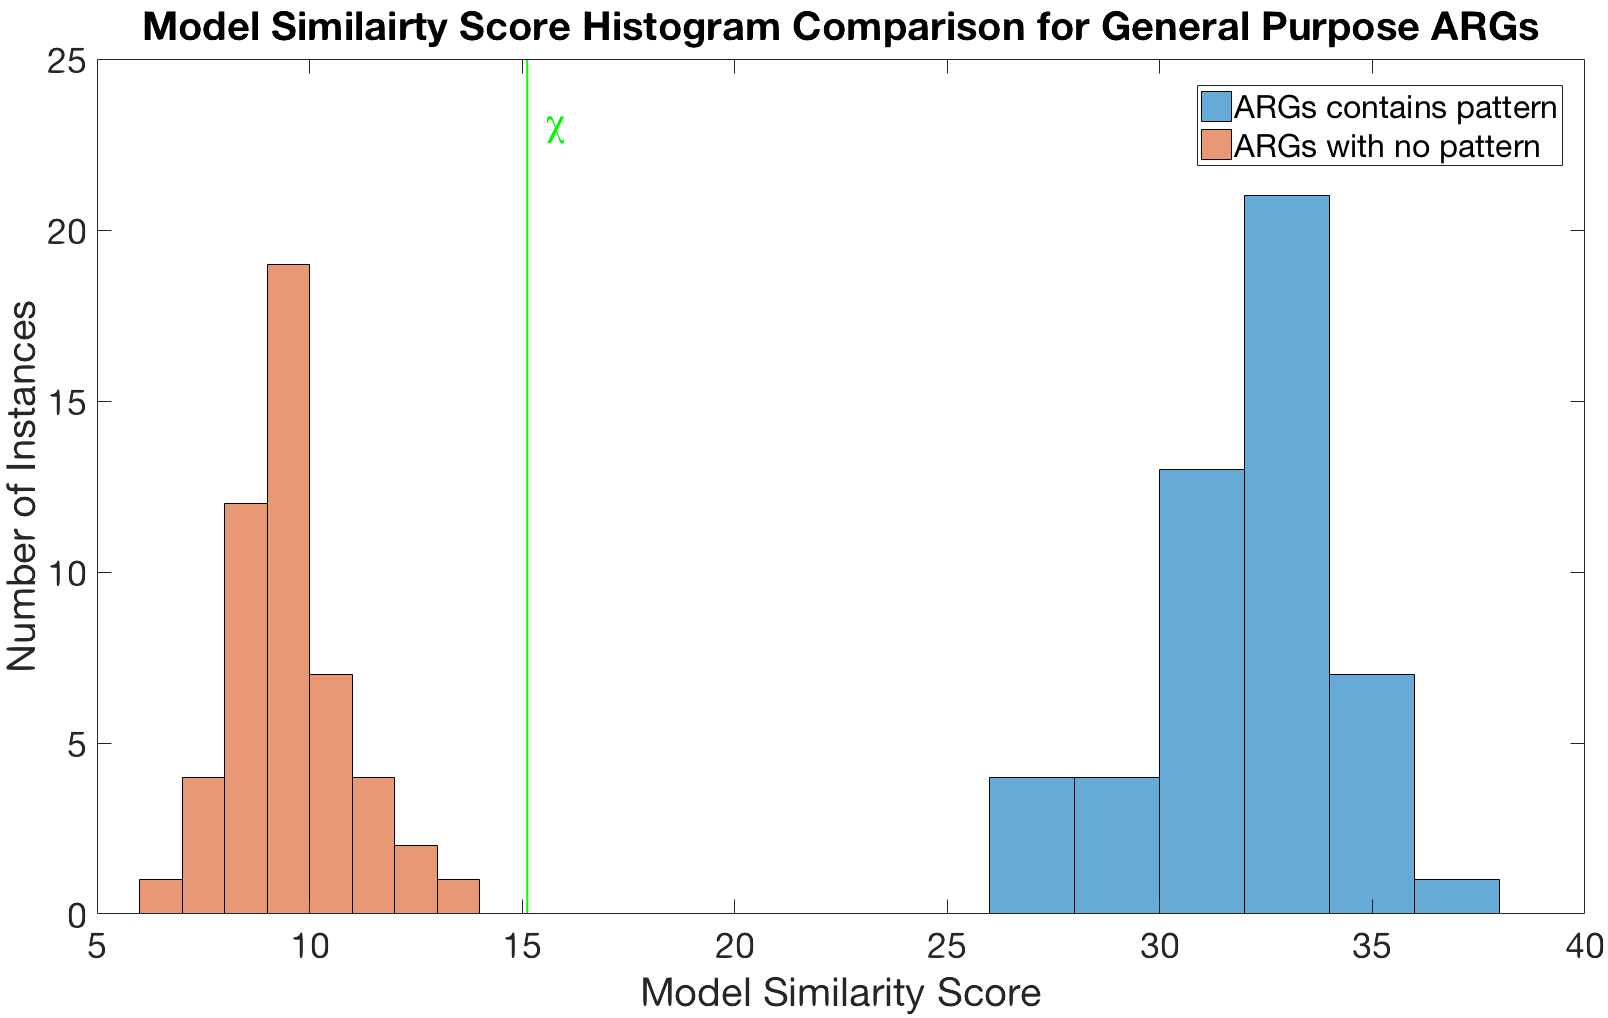
\includegraphics[width=0.9\textwidth]{figs/pattern_learning.png}
	\caption[Caption for LOF]{\emph{Similarity Score $f(G|Z)$ for pattern embedded ARG (blue) and random ARG(orange) while the green vertical line is the threshold $\chi$.}}
	\label{fig:pattern_learning}
\end{figure}

\section{Conclusion}

In this chapter we introduced a probabilistic parametric model $Z$ that we can train via EM algorithm. This model allows us to learn the common/share pattern among a set of ARGs, and used a set of component ARGs to represent/summarize such pattern. By calculating $f(G|Z)$ and comparing it to the threshold $\chi$, we can predict if a new ARG $G$ contains the learned pattern.\\

If we can model a protein crystal structure as an ARG, we can potentially use this model to mine novel protein structure or functional structure from protein crystallography data.







